\chapter{Conclusions}
\label{ch:conclusions}

This thesis presented a measurement of
the neutrino mixing angle \thetaot{}
using observation of reactor \nuebar{} disappearance
via the IBD reaction and neutron capture on hydrogen (nH)
at the Daya Bay experiment.
After introducing the history and theory of neutrino oscillations,
the Daya Bay experimental apparatus was described.
Precise characterization of the detector response
via a thorough calibration regime
constrained the possible variations between antineutrino detectors (ADs)
to the sub-percent level for most quantities.
The event-by-event position and energy reconstruction were used
to extract physically-meaningful quantities from the raw electronics data.
Event selection cuts were introduced to select an IBD-enriched sample
based on the double coincidence of positron annihilation and nH capture,
and the irreducible backgrounds were characterized via dedicated studies.
The selected events were used as input to a model
built on the premise of near-to-far projection,
where the observations at the near halls
were propagated to the far hall ADs
to determine the predicted event count based on an assumed value of \thetaot{}.
The model was fit to the observations using a $\chi^2$ expression
based on the Poisson maximum likelihood estimator
with nuisance parameters representing systematic uncertainties
as well as the statistical fluctuations at the near hall ADs.
The best-fit value of \thetaot{} was obtained by minimizing the $\chi^2$ expression
with respect to \thetaot{} and all pull parameters,
and the uncertainty and error budget were determined
using standard statistical techniques.
The result of $\sin^22\thetaot = 0.0731^{+0.0087}_{-0.0089}$
will be discussed in \cref{sec:discussion}.
Future prospects will be presented in \cref{sec:future}.

\section{Discussion}
\label{sec:discussion}

As shown in \cref{fig:theta13_vs_t_mine}, the nH-based measurements for $\sin^22\thetaot{}$,
including the result of this thesis, are approximately 0.01
less than the nGd-based measurements.
In particular, this thesis reports a measurement of $\sin^22\thetaot$
which is 1.4 standard deviations smaller
than the measurement in \cite{ngd2018} of
$\sin^22\thetaot = 0.0856\pm0.0029$.
A variety of potential resolutions to this discrepancy have been proposed
based on mis-characterizations of detection efficiencies, backgrounds,
or systematic biases present in the nH analysis but not in the nGd analysis.

\begin{figure}
    \centering
    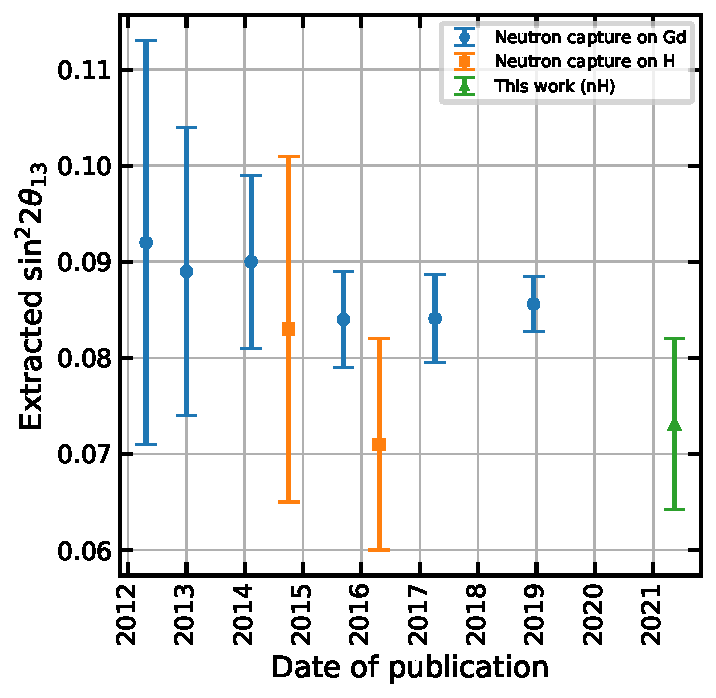
\includegraphics[width=0.9\textwidth]{ch_conclusion/theta13_vs_time_mine}
    \caption[This measurement compared to earlier results]{
        Published values of $\sin^{2}2\thetaot$ over time
        for both nGd and nH analyses by the Daya Bay experiment,
        including this measurement.
        Some nGd results were reported with separate statistical
        and systematic errors;
        those have been combined linearly for this plot.
    }
    \label{fig:theta13_vs_t_mine}
\end{figure}

The first avenue of investiation was the accidental background,
which had a rate at the far hall ADs greater than the signal IBD rate,
and at least 2 orders of magnitude greater than the rate
of any other irreducible background (see \cref{tab:summary_event_selection}).
This background was described in \cref{sec:acc}.
The method for determining the uncorrelated event rate
was validated using simulation in \cref{subsec:sim_singles}
to within \SI{0.017}{\percent}.
Accounting for the coincidence distance distribution of the accidental background
was more difficult.
\Cref{sec:DT_cut} describes studies made using double coincidences
rejected for having a DT value larger than \SI{800}{\mm},
which were assumed to be mostly accidentals.
A minimum DT value of \SI{3}{\m} was used to ensure no residual correlated events
were selected.
Based on the uncorrelated event rate and the synthetic accidentals sample,
the predicted number of these high-DT events matched the observation
to at worst \SI{0.04}{\percent}.
Due to the true correlated events at low DT, such a correspondence
was impossible to establish at lower DT values;
however, only in pathological situations
would the DT distribution of synthetic accidentals match the true distribution
at high DT values but diverge for lower DT values.
Thus the rate of accidental events in the final sample
was validated with a systematic uncertainty of \SI{0.04}{\percent},
just half of the statistical uncertainty of \SI{0.08}{\percent}.

The second potential source of major systematic bias for the nH analysis
was the efficiency of the DT cut, defined in \cref{eq:DT}.
While the coincidence time $\Delta t$ was measured precisely
using the \SI{\sim1}{\ns} precision of the readout electronics,
the coincidence distance $\Delta r$ was much less precise.
The reconstructed position had a resolution
of $\SI{\sim200}{\mm}$ for neutron captures
and \SI{\sim150}{\mm} for positrons \cite{adsimple1},
both of which were substantial fractions of the DT cut value of \SI{800}{\mm}.
Potential variations in the DT cut efficiency
were analyzed in \cref{sec:DT_cut}.
Although extracting the absolute DT cut efficiency
for the entire IBD data set proved difficult
due to presumed residual effects from subtracting the accidental background,
various subsets of events were successfully characterized,
all having AD-to-AD variations with a half-range smaller than
the \SI{0.5}{\percent} uncertainty used in this analysis.
One potential remaining cross-check to ensure the DT cut is treated correctly
is to search for a dependence of \thetaot{} on the value of the DT cut;
obviously, if the extracted value \thetaot{} changes
based on the value of this cut,
then there is a hidden bias that must be corrected.

A third category of potential biases
was the potential for unaccounted-for irredicuble backgrounds,
which in general change the apparent ratio of IBD event rates
between the near and far ADs and thus bias \thetaot{}.
The residual flasher events discussed in \cref{subsec:flash_resid}
were one such background which was discovered, characterized,
and rejected from the data sample using additional event selection cuts.
Ignoring this background would lead to an extracted value of $\sin^22\thetaot$
too large by approximately \num{0.003} (\SI{4}{\percent}).
Radiogenic neutrons due to radiocontaminants in the PMTs,
discussed in \cref{subsec:radn},
formed another background which was, until this analysis, neglected.
Although the characterization of the radiogenic neutron background rate
remains limited to Monte Carlo simulation studies \cite{rad_n},
neglecting this background with rate \num{0.2\pm0.1} per AD per day
resulted in a lower extracted value of $\sin^22\thetaot$
by almost \num{0.005} (\SI{7}{\percent}).

\section{Future prospects}
\label{sec:future}

The measurement of \thetaot{} by observation of neutron capture on hydrogen (nH)
is an important cross-check to the standard nGd measurement
since they are statistically-independent measurements and
have different contributions of backgrounds and systematic uncertainties.
Resolving the tension between the nH and nGd measurements of \thetaot{}
would build confidence in the final result.
Additional analysis work is also needed to measure $\Delta m^2_{32}$
based on the spectral shape of the nH data set.

\subsection{Resolving the nH-nGd tension}
\label{subsec:tension}

Additional investigation is planned to explain the continued discrepancy
of $\sim0.01$ between the nH and nGd extracted values of $\sin^22\thetaot$.
Many of the studies reported in \cref{ch:event_selection}
were designed to search for possible explanations for this tension.
Potential additional cross-checks include:
\begin{itemize}
    \item Does the value of the DT cut threshold affect the extracted value of
        \thetaot{}?
    \item Are the extracted values of \thetaot{} consistent when
        based only on data from a single run period (6-AD, 8-AD or 7-AD)?
    \item Does changing the position reconstruction algorithm
        change the extracted value of \thetaot{}?
    \item Does the extracted value of \thetaot{} depend on
        the value of the prompt energy cut lower bound?
\end{itemize}
These tests may help to identify an erroneous assumption
or AD-to-AD variation that has not previously been identified,
and would eventually lead to an updated measurement of \thetaot{}.


\subsection{Measuring \texorpdfstring{$\Delta m^2_{32}$}{the 3,2 mass splitting}}
\label{subsec:rateplusshape}

The near-to-far projection model described in \cref{sec:prediction}
already predicts both the rate and spectral shape
of the far hall AD observations,
and the fitter software has been validated using the same simulations
described in \cref{subsec:fitter_validation}
to ensure an accurate and unbiased value of $\Delta m^2_{32}$.
Remaining prerequisites for a successful rate plus shape analysis
include resolution of the above tension based solely on the IBD rates,
as well as an improved characterization of the ADs' energy response.
Specifically, while the uniformity of the energy response
as a function of event position
has been thoroughly measured and constrained within the GdLS volume,
the observed nonuniformity in the LS region
has much larger variations across ADs
and is not stable when measured using different methodologies \cite{beda_nonuniformity}.
Without a better constraint on the energy response,
the spectral shape could be distorted in poorly-understood ways,
leading to an incorrect measurement of $\Delta m^2_{32}$.
